\documentclass{article}
\usepackage[paper=letterpaper,margin=2cm]{geometry}
\usepackage[utf8]{inputenc}
\usepackage[russian]{babel}
\usepackage[]{graphicx}
\usepackage[usenames]{color}
\usepackage{colortbl}
\usepackage{geometry}
\usepackage{xcolor}
\usepackage{hyperref}
\usepackage{../../lib/latex/listings-rust}
\usepackage{fontspec}
\setmonofont{JetBrains Mono}[Contextuals=Alternate,Ligatures = TeX,]
\usepackage{listings}
\usepackage{keycommand}
\usepackage{caption}

\setmainfont[
  Ligatures=TeX,
  Extension=.otf,
  BoldFont=cmunbx,
  ItalicFont=cmunti,
  BoldItalicFont=cmunbi,
]{cmunrm}
\setsansfont[
  Ligatures=TeX,
  Extension=.otf,
  BoldFont=cmunsx,
  ItalicFont=cmunsi,
]{cmunss}

\geometry{
  a4paper,
  top=25mm,
  right=30mm,
  bottom=25mm,
  left=30mm
}

\hypersetup{
  colorlinks=true,
  linkcolor=blue!50!red,
  urlcolor=blue!70!black
}

\captionsetup[lstlisting]{
  font={tt},
}

% based on Atom One Light
\lstset{
  language=Java,
  frame=single,
  basicstyle=\ttfamily\color[HTML]{383a42},
  columns=fullflexible,
  breaklines=true,
  numbers=left,
  frame=tab,
  postbreak=\mbox{\textcolor{red}{$\hookrightarrow$}\space},
  extendedchars=false,
  showspaces=false,
  showstringspaces=false,
  identifierstyle=\ttfamily\color[HTML]{4078f2},
  commentstyle=\color[HTML]{a0a1a7},
  stringstyle=\color[HTML]{50a14f},
  keywordstyle=\color[HTML]{a626a4},
  numberstyle=\ttfamily\color[HTML]{2c91af},
  rulecolor=\color[HTML]{383a42}
}

\lstdefinelanguage{XML}
{
  morestring=[b]",
  morestring=[s]{>}{<},
  morecomment=[s]{<?}{?>},
}

\newcommand{\code}[1]{
  \lstset{title=#1}
  \lstinputlisting{#1}
}
\newkeycommand{\itmo}[variant=aboba, labn=aboba, discipline=aboba, group=aboba, student=aboba,teacher=aboba, year=2022]{
  \begin{titlepage}
    \begin{center}
      \section*{
        Федеральное государственное автономное образовательное учреждение\\ высшего образования\\
        «Национальный исследовательский университет ИТМО»\\
        Факультет Программной Инженерии и Компьютерной Техники \\
       }
      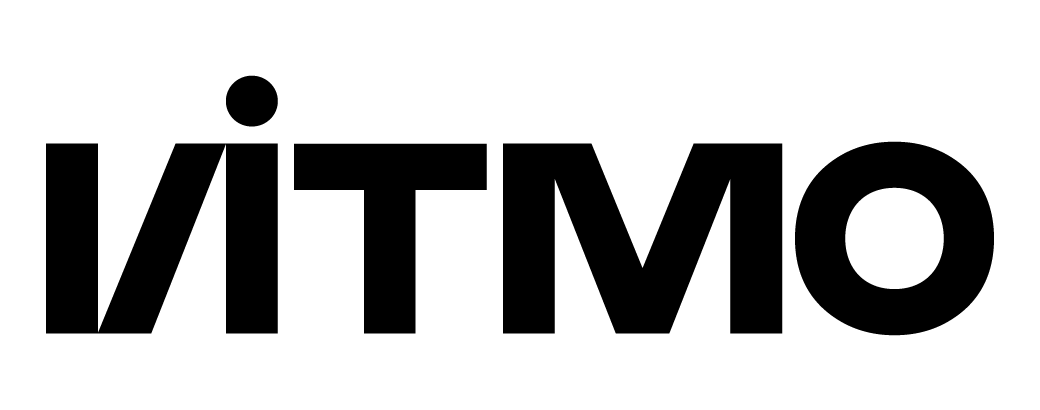
\includegraphics[scale=0.2]{../../lib/img/itmo.png}
    \end{center}

    \vspace{4cm}

    \begin{center}
      \large \textbf{Вариант \textnumero \commandkey{variant}}\\
      \textbf{Лабораторная работа \textnumero \commandkey{labn}}\\
      по дисциплине\\
      \textbf{\commandkey{discipline}}
    \end{center}

    \vspace*{\fill}

    \begin{flushright}
      Выполнил Студент группы \commandkey{group}\\
      \textbf{\commandkey{student}}\\
      Преподаватель: \\
      \textbf{\commandkey{teacher}}\\
    \end{flushright}

    \vspace{1cm}

    \begin{center}
      г. Санкт-Петербург\\
      \commandkey{year}г.
    \end{center}

    \thispagestyle{empty}
  \end{titlepage}
}


\begin{document}

\itmo[
  variant=1500235,
  labn=2,
  discipline=Программирование,
  group=P3115,
  student=Владимир Мацюк,
  teacher=Сорокин Роман Борисович
]

\tableofcontents

\section{Текст задания}

\begin{enumerate}
  \item На основе базового класса Pokemon написать свои классы для заданных видов покемонов. Каждый вид покемона должен иметь один или два типа и стандартные базовые характеристики:
        \begin{itemize}
          \item очки здоровья (HP)
          \item атака (attack)
          \item защита (defense)
          \item специальная атака (special attack)
          \item специальная защита (special defense)
          \item скорость (speed)
        \end{itemize}
  \item Классы покемонов должны наследоваться в соответствии с цепочкой эволюции покемонов. На основе базовых классов PhysicalMove, SpecialMove и StatusMove реализовать свои классы для заданных видов атак.
        
  \item Атака должна иметь стандартные тип, силу (power) и точность (accuracy). Должны быть реализованы стандартные эффекты атаки. Назначить каждому виду покемонов атаки в соответствии с вариантом. Уровень покемона выбирается минимально необходимым для всех реализованных атак.
        
  \item Используя класс симуляции боя Battle, создать 2 команды покемонов (каждый покемон должен иметь имя) и запустить бой.
        
  \item Базовые классы и симулятор сражения находятся в \href{https://se.ifmo.ru/documents/10180/660917/Pokemon.jar/a7ce60af-6ee6-47d0-a95e-e5ed9a697bd2}{jar-архиве} (обновлен 9.10.2018, исправлен баг с добавлением атак и кодировкой). Документация в формате javadoc - \href{https://se.ifmo.ru/~tony/doc/}{здесь}.
        
  \item Информацию о покемонах, цепочках эволюции и атаках можно найти на сайтах \url{http://poke-universe.ru}, \url{http://pokemondb.net}, \url{http://veekun.com/dex/pokemon}
\end{enumerate}

\section{Комментарии}
\begin{enumerate}
  \item Ознакомиться с документацией, обращая особое внимание на классы Pokemon и Move. При дальнейшем выполнении лабораторной работы читать документацию еще несколько раз.
  \item Скачать файл Pokemon.jar. Его необходимо будет использовать как для компиляции, так и для запуска программы. Распаковывать его не надо! Нужно научиться подключать внешние jar-файлы к своей программе.
  \item Написать минимально работающую программу и посмотреть как она работает.
        \begin{lstlisting}
Battle b = new Battle();
Pokemon p1 = new Pokemon("Чужой", 1);
Pokemon p2 = new Pokemon("Хищник", 1);
b.addAlly(p1);
b.addFoe(p2);
b.go();
\end{lstlisting}
  \item Создать один из классов покемонов для своего варианта. Класс должен наследоваться от базового класса Pokemon. В конструкторе нужно будет задать типы покемона и его базовые характеристики. После этого попробуйте добавить покемона в сражение.
  \item Создать один из классов атак для своего варианта (лучше всего начать с физической или специальной атаки). Класс должен наследоваться от класса PhysicalMove или SpecialMove. В конструкторе нужно будет задать тип атаки, ее силу и точность. После этого добавить атаку покемону и проверить ее действие в сражении. Не забудьте переопределить метод describe, чтобы выводилось нужное сообщение.
  \item Если действие атаки отличается от стандартного, например, покемон не промахивается, либо атакующий покемон также получает повреждение, то в классе атаки нужно дополнительно переопределить соответствующие методы (см. документацию). При реализации атак, которые меняют статус покемона (наследники StatusMove), скорее всего придется разобраться с классом Effect. Он позволяет на один или несколько ходов изменить состояние покемона или модификатор его базовых характеристик.
  \item Доделать все необходимые атаки и всех покемонов, распределить покемонов по командам, запустить сражение.
\end{enumerate}

\section{Покемоны}
\begin{center}
  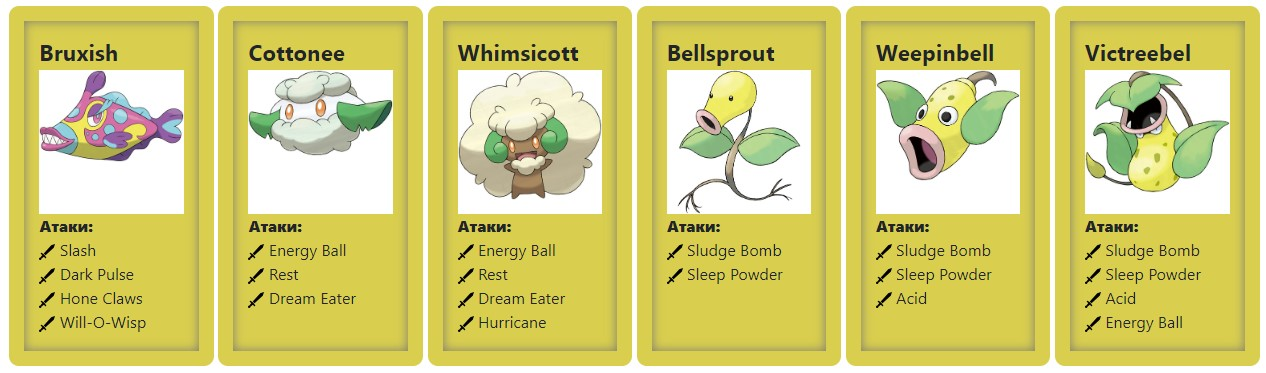
\includegraphics[scale=0.5]{pokemons.jpg}
\end{center}

\section{Диаграмма классов}

\begin{center}
  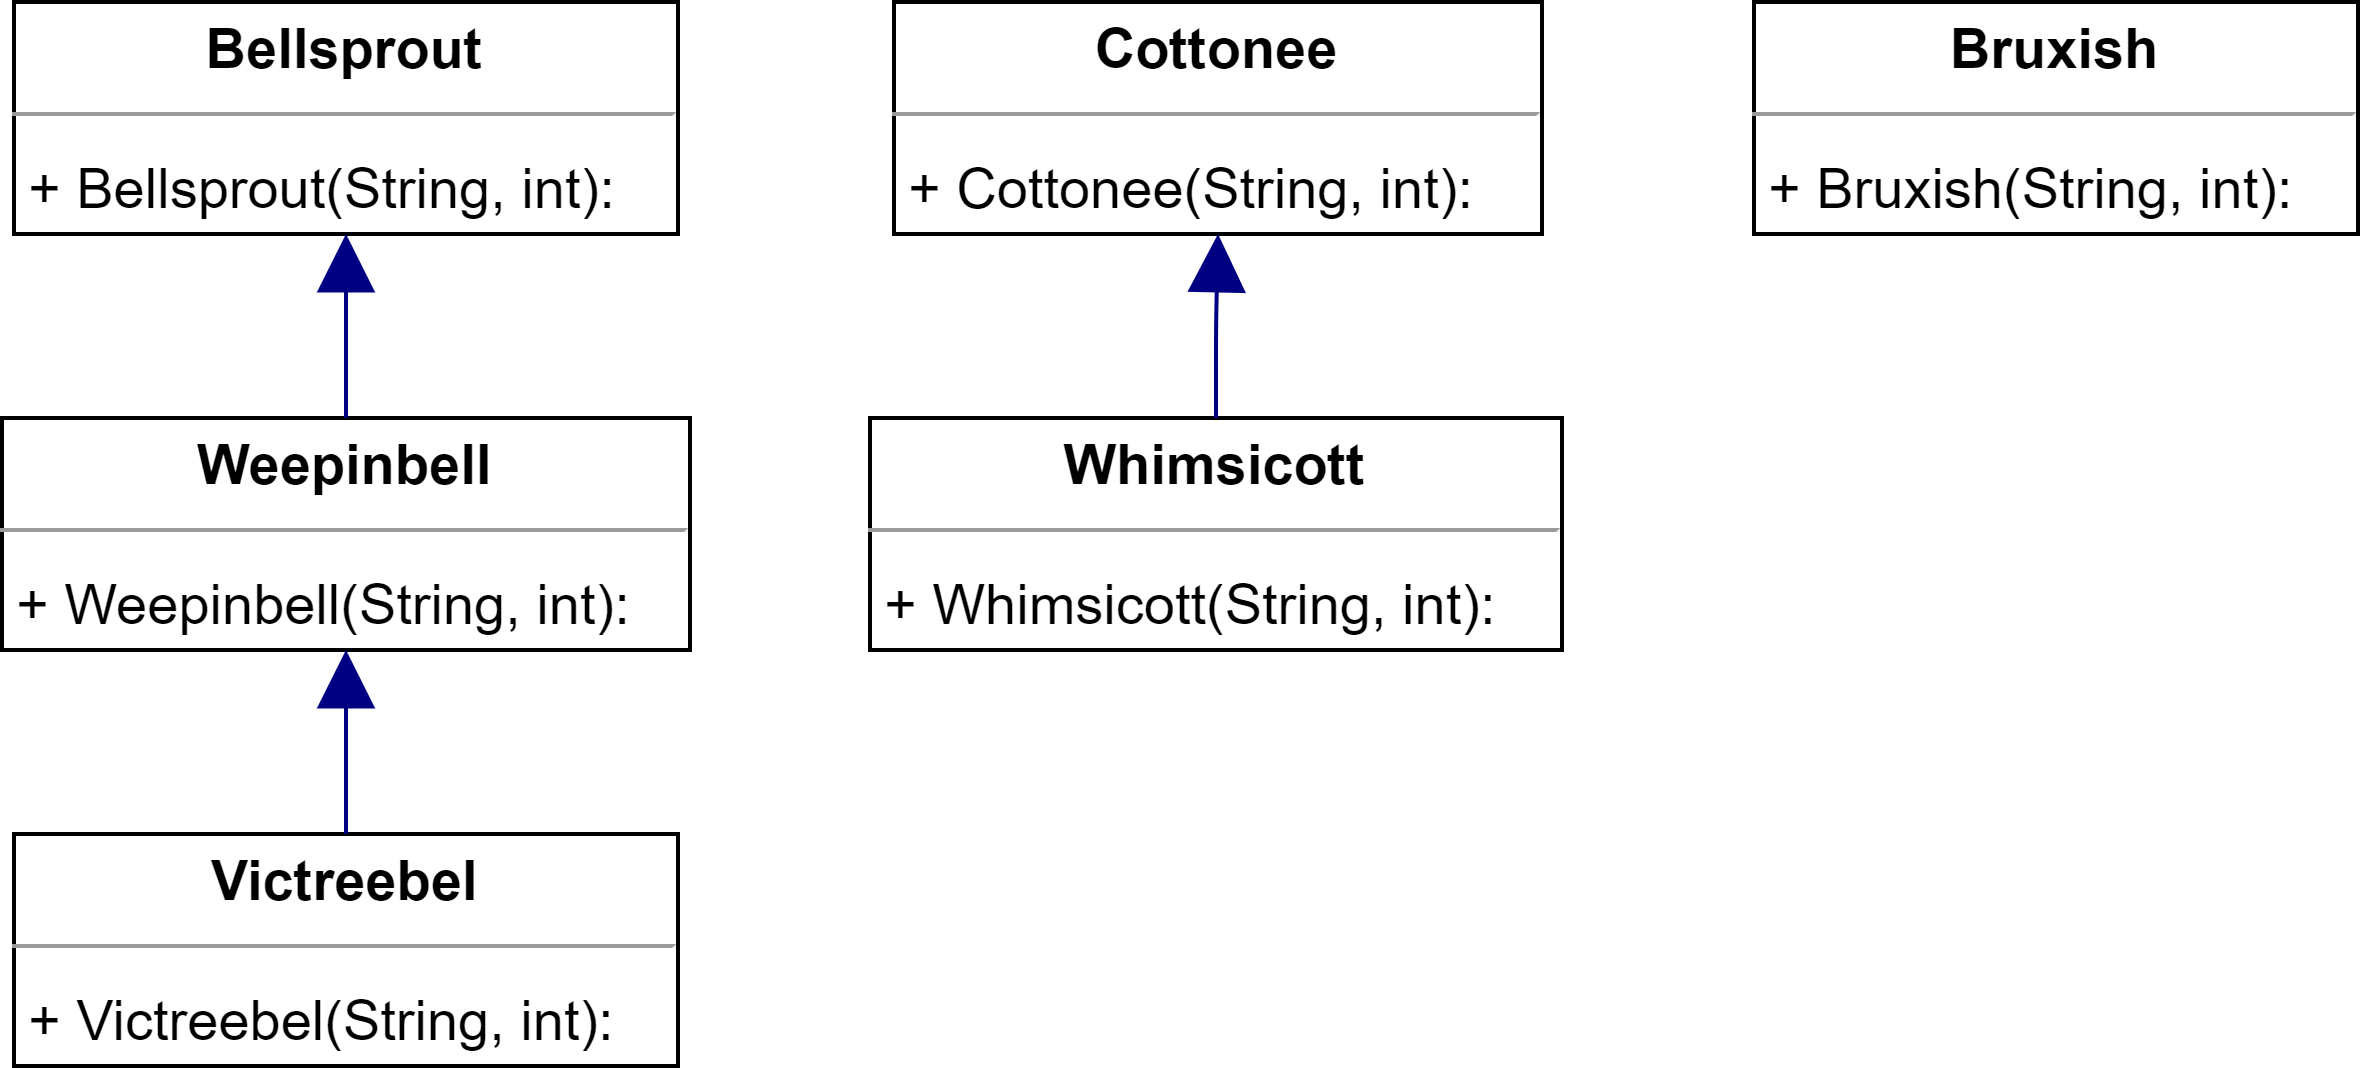
\includegraphics[scale=0.2]{diagram.png}
\end{center}

\section{Ссылка на github}
\url{https://github.com/Wgmlgz/itmo/tree/main/prog/lab2}
\section{Результат работы программы}
\lstset{ basicstyle=\ttfamily\color[HTML]{383a42}}
\code{out.txt}
\section{Вывод}
Во время выполнения работы я ознакомился с ООП на языке java. Научился разрабатывать архитектуру проекта и подключать jar архивы к проекту.
\end{document}
